%%%%%%%%%%%%%%%%%%%%%%%%%%%%%%%%%%%%%%%%%%%%%%%%%%%%%%%%%%%%%%%%%%%%%
%                                                                   %
%              Major Project Final Report -- MetaJudge-AI          %
%       Formatted for BVCOE (Dept. of IT) -- WITH FIGURES          %
%                                                                   %
%%%%%%%%%%%%%%%%%%%%%%%%%%%%%%%%%%%%%%%%%%%%%%%%%%%%%%%%%%%%%%%%%%%%%

\documentclass[12pt, a4paper]{report}

% ----------------------------------------------------------------- %
%  A. PACKAGE IMPORTS
% ----------------------------------------------------------------- %
\usepackage[a4paper, left=1.5in, right=1in, top=1in, bottom=1in]{geometry}
\usepackage{graphicx}
\usepackage{times}
\usepackage{setspace}
\usepackage{amsmath, amssymb}
\usepackage[nottoc,notlot,notlof]{tocbibind}
\usepackage{longtable}
\usepackage{array}
\usepackage{enumitem}
\usepackage{tabularx}
\usepackage{multirow}
\usepackage{booktabs}
\usepackage[table]{xcolor}
\usepackage{listings}
\usepackage{hyperref}
\usepackage{tikz}
\usepackage{pgfplots}
\usepackage{pgfplotstable}
\pgfplotsset{compat=1.18}
\usetikzlibrary{shapes.geometric, arrows.meta, positioning,
                fit, backgrounds, decorations.pathreplacing, calc}
\usepackage{titlesec}
\usepackage{fancyhdr}

\hypersetup{
    colorlinks=true,
    linkcolor=black,
    filecolor=magenta,
    urlcolor=blue,
    pdftitle={Major Project Final Report -- MetaJudge-AI},
    pdfpagemode=FullScreen,
}

% ----------------------------------------------------------------- %
%  BVCOE HEADING SIZES
% ----------------------------------------------------------------- %
\titleformat{\chapter}[display]
  {\normalfont\fontsize{18}{22}\bfseries\centering}
  {\chaptertitlename\ \thechapter}{12pt}{}
\titleformat{\section}
  {\normalfont\fontsize{16}{20}\bfseries}{\thesection}{1em}{}
\titleformat{\subsection}
  {\normalfont\fontsize{14}{18}\bfseries}{\thesubsection}{1em}{}
\titleformat{\subsubsection}
  {\normalfont\fontsize{12}{16}\bfseries}{\thesubsubsection}{1em}{}

% --- Custom Colors & Styles ---
\definecolor{bvblue}{RGB}{31,56,100}
\definecolor{ltblue}{RGB}{46,117,182}
\definecolor{rowgray}{RGB}{242,242,242}
\definecolor{codegreen}{rgb}{0,0.5,0}
\definecolor{myblue}{RGB}{31,78,153}
\definecolor{mygreen}{RGB}{0,112,44}
\definecolor{myorange}{RGB}{197,90,17}
\definecolor{mygray}{RGB}{89,89,89}

\lstdefinestyle{pycode}{
    backgroundcolor=\color{rowgray},
    commentstyle=\color{codegreen},
    keywordstyle=\color{bvblue},
    basicstyle=\ttfamily\footnotesize,
    breakatwhitespace=false,
    breaklines=true,
    keepspaces=true,
    showspaces=false,
    showstringspaces=false,
    frame=single,
    rulecolor=\color{ltblue},
    xleftmargin=10pt,
    xrightmargin=10pt,
    language=Python,
}

\newcolumntype{L}[1]{>{\raggedright\arraybackslash}p{#1}}
\newcolumntype{C}[1]{>{\centering\arraybackslash}p{#1}}
\newcolumntype{R}[1]{>{\raggedleft\arraybackslash}p{#1}}

\newcommand{\sys}{\textsc{MetaJudge-AI}}

% ----------------------------------------------------------------- %
%  B. DOCUMENT START
% ----------------------------------------------------------------- %
\begin{document}

% ================================================================= %
%  TITLE PAGE
% ================================================================= %
\begin{titlepage}
    \centering

    {\fontsize{20}{24}\selectfont\onehalfspacing
    \textbf{Meta-Verification of LLM Judges through Adversarial Falsification for Hallucination Correction}}
    \vspace{0.5cm}

    {\fontsize{12}{14}\bfseries MAJOR PROJECT -- DISSERTATION}
    \vspace{0.4cm}

    {\fontsize{12}{14}\selectfont\itshape
    submitted in partial fulfillment of the requirements for the award of the degree of}
    \vspace{0.3cm}

    {\fontsize{14}{18}\bfseries BACHELOR OF TECHNOLOGY}
    \vspace{0.1cm}

    {\fontsize{12}{14}\itshape in}
    \vspace{0.2cm}

    {\fontsize{14}{18}\bfseries DEPARTMENT OF INFORMATION TECHNOLOGY}
    \vspace{0.5cm}

    {\fontsize{12}{14}\itshape Submitted by}
    \vspace{0.3cm}

    {\fontsize{12}{14}\bfseries
    Ayush Sharma \\
    05611503122}
    \vspace{0.5cm}

    {\fontsize{12}{14}\itshape\bfseries Under the supervision of}
    \vspace{0.3cm}

    {\fontsize{12}{14}\bfseries
    Ms. Neetu Singh \\
    Assistant Professor, Information Technology}

    \vspace{0.6cm}

    % Logo in the middle of the page, between supervisor and institution.
    % A framed placeholder is used if the image file is unavailable.
    \IfFileExists{bvcoe_logo.jpeg}{%
        \includegraphics[width=0.45\textwidth]{bvcoe_logo.jpeg}%
    }{%
        \fbox{\parbox[c][3cm][c]{0.45\textwidth}{\centering BVCOE Logo}}%
    }

    \vspace{0.5cm}

    {\fontsize{12}{14}\bfseries
    DEPARTMENT OF INFORMATION TECHNOLOGY \\
    BHARATI VIDYAPEETH'S COLLEGE OF ENGINEERING \\}
    {\fontsize{12}{14}\selectfont
    (AFFILIATED TO GURU GOBIND SINGH INDRAPRASTHA UNIVERSITY, DELHI) \\
    NEW DELHI -- 110063 \\}
    \vspace{0.2cm}
    {\fontsize{12}{14}\bfseries MAY / JUNE 2026}
\end{titlepage}
% ================================================================= %
%  CERTIFICATE
% ================================================================= %
\newpage
\thispagestyle{empty}
\pagenumbering{roman}
\setcounter{page}{2}

\begin{center}
    {\fontsize{16}{20}\bfseries CERTIFICATE}
\end{center}
\vspace{1cm}
\onehalfspacing

\noindent
This is to certify that the work embodied in this Major Project -- Dissertation titled
\textbf{``Meta-Verification of LLM Judges through Adversarial Falsification for Hallucination Correction''} being submitted in the partial fulfillment of the
requirements for the award of the degree of \textbf{Bachelor of Technology} in
\textbf{Information Technology}, is original and has been carried out by
\textbf{Ayush Sharma} (Enrollment No.\ 05611503122) under my supervision and
guidance.

\vspace{0.5cm}
\noindent
It is further certified that this Major Project -- Dissertation work has not been
submitted in full or in part to this university or any other university for the award
of any other degree or diploma to the best of my knowledge and belief.

\vspace{2.5cm}
\noindent
\begin{tabular}{p{0.45\textwidth} p{0.45\textwidth}}
\textbf{(Ms. Neetu Singh)} & \textbf{(Dr. Prakhar Priyadarshi)} \\
Project Supervisor                 & Head of Department \\
Assistant Professor, Dept.\ of IT            & Dept.\ of Information Technology \\
BVCOE, New Delhi                   & BVCOE, New Delhi \\
\end{tabular}

\vspace{2cm}
\noindent
\textbf{External Examiner:} \hrulefill

\vspace{0.5cm}
\noindent
\textbf{Date:} \hrulefill

% ================================================================= %
%  CANDIDATE'S DECLARATION
% ================================================================= %
\newpage
\thispagestyle{empty}
\begin{center}
    {\fontsize{16}{20}\bfseries CANDIDATE'S DECLARATION}
\end{center}
\vspace{1cm}
\doublespacing

\noindent
This is to certify that the material embodied in this Major Project -- Dissertation
titled \textbf{``Meta-Verification of LLM Judges through Adversarial Falsification for Hallucination Correction''} being submitted in the partial fulfillment of the
requirements for the award of the degree of \textbf{Bachelor of Technology} in
\textbf{Information Technology} is based on my original work. It is further certified
that this Major Project -- Dissertation work has not been submitted in full or in part
to this university or any other university for the award of any other degree or diploma.
My indebtedness to other works has been duly acknowledged at the relevant places.

\vspace{3cm}
\begin{flushright}
\textbf{Ayush Sharma} \\
\textbf{05611503122}
\end{flushright}

% ================================================================= %
%  ACKNOWLEDGEMENT
% ================================================================= %
\newpage
\thispagestyle{empty}
\begin{center}
    {\fontsize{16}{20}\bfseries ACKNOWLEDGEMENT}
\end{center}
\vspace{1cm}
\onehalfspacing

\noindent
I would like to express my sincere gratitude to \textbf{Ms. Neetu Singh},
Assistant Professor, Department of Information Technology, Bharati
Vidyapeeth's College of Engineering, New Delhi, for her invaluable guidance,
continuous encouragement, and constructive feedback throughout the course of this
project.

\vspace{0.5cm}
\noindent
I am thankful to the faculty members of the Department of Information Technology,
BVCOE, for their support and suggestions. I also extend my thanks to Bharati
Vidyapeeth's College of Engineering for providing the necessary infrastructure and
resources.

\vspace{0.5cm}
\noindent
Finally, I thank my family and friends for their unwavering support and motivation
during this project.

\vspace{2cm}
\begin{flushright}
\textbf{Ayush Sharma} \\
\textbf{05611503122}
\end{flushright}

% ================================================================= %
%  ABSTRACT
% ================================================================= %
\newpage
\thispagestyle{empty}
\begin{center}
    {\fontsize{16}{20}\bfseries ABSTRACT}
\end{center}
\vspace{1cm}
\onehalfspacing

\noindent
\sys{} is a hallucination detection and correction framework for AI-generated
summaries of AI/ML research papers. The project is motivated by a practical
failure mode of retrieval-augmented generation (RAG): a search query that asks
whether a claim is true often retrieves semantically related support even when
the specific value, date, author, venue, or benchmark result is wrong. \sys{}
therefore reframes verification as adversarial falsification. Instead of asking
``find evidence for this claim'', it asks the retrieval system to find evidence
that the claim is false, then verifies any correction through a second
meta-judgment step.

\vspace{0.4cm}
\noindent
The implemented system follows a six-stage pipeline: atomic claim
decomposition, cross-claim consistency checking, adversarial query generation,
hybrid retrieval, LLM judging with Chain-of-Verification (CoVe)
meta-verification, and surgical correction. Retrieval combines direct arXiv
lookup, adversarial arXiv search, web search, Semantic Scholar fallback, cached
evidence, and optional PDF-level extraction for numeric claims. The CoVe loop is
applied to the judge rather than to the original answer: when the judge claims a
contradiction, it must ground that contradiction in a real evidence quote before
the editor is allowed to change the summary.

\vspace{0.4cm}
\noindent
The evaluation uses the available SkepticBench sample of five papers, containing
three corrupted summaries and two clean summaries. On this sample, full
\sys{} achieves F1 = 0.800, Precision = 1.000, and Recall = 0.667, with zero
false positive corrections. Removing the CoVe loop increases recall to 1.000
and F1 to 0.857 but introduces a false positive (Precision = 0.750). Removing
adversarial queries lowers F1 to 0.500 and Recall to 0.333, a 37.5\% drop in
F1 relative to the full system. These results support the central thesis that
adversarial falsification is more effective than confirmatory retrieval for
detecting factual errors, while CoVe provides a conservative precision gate that
is appropriate for correction systems where false edits are costly.
\vspace{0.4cm}
\noindent
The main contribution is an end-to-end, reproducible prototype that combines
skeptical retrieval, judge verification, and minimal editing for scientific
summaries. The report also states the limitations honestly: the validated run is
small, external baselines are contextual rather than directly benchmarked on the
same sample, and retrieval quality remains constrained by abstracts, rate
limits, and provider availability.
% ================================================================= %
%  FRONT-MATTER LISTS
% ================================================================= %
\newpage
\listoftables
\cleardoublepage
\listoffigures
\cleardoublepage

% ----------------------------------------------------------------- %
%  LIST OF SYMBOLS AND ABBREVIATIONS
% ----------------------------------------------------------------- %
\newpage
\begin{center}
    {\fontsize{16}{20}\bfseries LIST OF ABBREVIATIONS}
\end{center}
\vspace{1cm}
\onehalfspacing

\begin{tabular}{L{3cm} L{9cm}}
\toprule
\textbf{Abbreviation} & \textbf{Description} \\
\midrule
AI & Artificial Intelligence \\
RAG & Retrieval-Augmented Generation \\
LLM & Large Language Model \\
CoVe & Chain-of-Verification \\
NIM & NVIDIA Inference Microservice \\
API & Application Programming Interface \\
NLP & Natural Language Processing \\
RARR & Researching and Revising What Language Models Say, Using Language Models \\
SkepticBench & Benchmark Dataset for Scientific Summary Hallucination Evaluation \\
FastAPI & Modern Web Framework for Building APIs with Python \\
JSON & JavaScript Object Notation \\
CSV & Comma-Separated Values \\
PDF & Portable Document Format \\
SQLite & Lightweight Relational Database Used for Evidence Caching \\
HTTP & HyperText Transfer Protocol \\
REST & Representational State Transfer \\
FPR & False Positive Rate \\
\bottomrule
\end{tabular}

\cleardoublepage

\newpage
\begin{center}
    {\fontsize{16}{20}\bfseries LIST OF SYMBOLS}
\end{center}
\vspace{1cm}
\onehalfspacing

\begin{tabular}{L{3cm} L{9cm}}
\toprule
\textbf{Symbol / Abbreviation} & \textbf{Description} \\
\midrule
$N$ & Number of evaluated papers or claims \\
$TP$ & True positives: corrupted summaries correctly detected \\
$FP$ & False positives: clean summaries incorrectly flagged \\
$FN$ & False negatives: corrupted summaries missed by the system \\
$TN$ & True negatives: clean summaries correctly left unchanged \\
$P$ & Precision, $TP/(TP+FP)$ \\
$R$ & Recall, $TP/(TP+FN)$ \\
$F1$ & Harmonic mean of precision and recall \\
$FPR$ & False positive rate, $FP/(FP+TN)$ \\
$k$ & Number of retrieved evidence items or top search results \\
$\tau$ & Confidence or evidence threshold used by verification gates \\
\bottomrule
\end{tabular}

\cleardoublepage

% ----------------------------------------------------------------- %
%  TABLE OF CONTENTS
% ----------------------------------------------------------------- %
\tableofcontents
\cleardoublepage

% ================================================================= %
%  MAIN BODY
% ================================================================= %
\pagenumbering{arabic}
\onehalfspacing

% ================================================================= %
%  CHAPTER 1: INTRODUCTION
% ================================================================= %
\chapter{Introduction}

\section{Background and Motivation}

Large language models are increasingly used to summarize scientific papers,
compare benchmarks, and generate literature-review style explanations. In this
setting, hallucinations are often subtle: a model may state the wrong benchmark
score, year, author group, model size, training objective, or venue while keeping
the rest of the paragraph fluent and plausible. Such errors are risky because
they can propagate into surveys, project reports, research prototypes, and
downstream decisions.

Retrieval-Augmented Generation (RAG) is a common response to this problem, but
standard retrieval can become confirmatory. If the claim says ``BERT achieved
80.5\% F1 on SQuAD 2.0'', a query that simply repeats the claim may return
general BERT or SQuAD documents without forcing a comparison against the correct
number. \sys{} is motivated by the opposite strategy: a verifier should actively
try to falsify the claim, then allow a correction only when the contradiction is
grounded in explicit evidence.

\section{Project Overview}

\sys{} is a Python-based framework for hallucination detection and correction in
AI/ML paper summaries. It decomposes a summary into atomic facts, checks whether
claims contradict each other internally, generates adversarial search queries,
retrieves evidence from paper-centric sources, asks an LLM judge to classify each
claim, verifies the judge's own contradiction decision through CoVe, and applies
minimal corrections to the original summary.

The project is implemented as both a command-line pipeline and a FastAPI backend.
The LLM calls route through NVIDIA NIM using an OpenAI-compatible client. The
retrieval stack includes arXiv direct lookup, arXiv search, DuckDuckGo/DDGS web
search, Semantic Scholar fallback, PDF extraction for numeric claims, and SQLite
caching for rate-limit protection. The evaluation focuses on SkepticBench, a
paper-summary benchmark with explicit injected factual corruptions.

\section{Scope and Applicability}

The scope of the project is deliberately narrow and measurable. \sys{} is aimed
at English-language summaries of AI/ML research papers, especially claims about
authors, years, model names, training methods, benchmarks, and quantitative
results. It is suitable for batch review of generated summaries, report drafts,
and literature-review notes where preserving the original wording is important.

The current implementation is not a general-purpose misinformation detector. It
does not process images, audio, video, or multilingual documents, and it is not
designed for real-time social-media monitoring. Its strongest applicability is in
research-assistance workflows where factual precision and low false correction
rates matter more than maximum recall.

\section{Report Organisation}

Chapter 2 defines the problem and reviews related work in factuality evaluation,
RAG, CoVe, RARR, atomic fact checking, and LLM-as-judge reliability. Chapter 3
describes the proposed methodology and system architecture. Chapter 4 explains
the SkepticBench evaluation setup, metrics, and ablation conditions. Chapter 5
presents the experimental results and analysis. Chapter 6 discusses the meaning
of the results and the limitations of the current implementation. Chapter 7
concludes the report and identifies future work.



% ================================================================= %
%  CHAPTER 2: PROBLEM STATEMENT & LITERATURE
% ================================================================= %
\chapter{Problem Statement and Literature Survey}

\section{Problem Definition}

\subsection{Problem Identification}

The central problem is the reliable correction of factual errors in generated
scientific summaries. A correction system faces a stricter requirement than a
detection-only system: a false positive does not merely produce a wrong label,
it can actively damage a correct summary. Existing RAG-style systems often
retrieve relevant-looking support, but relevance is not the same as
contradiction. Existing LLM judges can also hallucinate their own verdicts by
claiming that evidence contradicts a statement without providing an exact
supporting quote.

The project therefore treats hallucination correction as a meta-verification
problem. The system must verify the generated summary, verify the evidence used
by the judge, and verify that a proposed edit is justified before modifying the
text.

\subsection{Objectives}

The primary objective is to build and evaluate a skeptical hallucination
correction pipeline for AI/ML paper summaries. Specific objectives include:

\begin{itemize}
    \item Decompose generated summaries into atomic, self-contained claims.
    \item Generate adversarial, falsification-oriented search queries instead of confirmatory search queries.
    \item Retrieve evidence from authoritative and practical sources such as arXiv, Semantic Scholar, web search, and paper PDFs.
    \item Use an LLM judge to classify claims as \texttt{SUPPORTED}, \texttt{CONTRADICTED}, or \texttt{INSUFFICIENT\_EVIDENCE}.
    \item Apply CoVe meta-verification to contradiction verdicts so that unsupported judge claims are overturned.
    \item Apply surgical corrections only when contradiction evidence survives verification.
    \item Quantify component contributions using ablation studies on the available SkepticBench sample.
\end{itemize}

\subsection{Research Questions}

The project addresses the following key research questions:

\begin{itemize}
    \item Does adversarial falsification improve hallucination detection compared with confirmatory retrieval?
    \item How does CoVe change the precision--recall trade-off for a correction system?
    \item Can cross-claim consistency checking identify contradictions that retrieval may miss?
    \item Can a surgical editor correct only the wrong span while preserving the rest of the generated summary?
    \item What limitations arise when the evaluation is constrained by API rate limits and a small validated benchmark sample?
\end{itemize}

\subsection{Scope and Limitations}

The scope is restricted to textual AI/ML paper summaries. The validated
evaluation uses five SkepticBench papers: three with injected factual errors and
two clean summaries. The repository also contains a larger CSV of approximately
1.4k entries, but the report does not claim full-scale evaluation over that file
because the available result artifact is the five-paper ablation run. The system
depends on external retrieval services and NVIDIA NIM model calls; therefore,
results can vary with provider availability, rate limits, cache state, and
retrieved evidence quality.


\section{Literature Survey Table}
    \begin{longtable}{|p{0.8cm}|p{3.5cm}|p{4.0cm}|p{3.5cm}|p{2.5cm}|}
    \caption{Literature Survey: From Supportive RAG to Skeptical Verification} \label{tab:literature_survey} \\
    \hline
    \textbf{S.N.} & \textbf{Paper Name} & \textbf{Core Methodology} & \textbf{Key Conclusions} & \textbf{Gap We Fill} \\
    \hline
    \endfirsthead
    \multicolumn{5}{c}%
    {{\bfseries \tablename\ \thetable{} -- continued from previous page}} \\
    \hline
    \textbf{S.N.} & \textbf{Paper Name} & \textbf{Core Methodology} & \textbf{Key Conclusions} & \textbf{Gap We Fill} \\
    \hline
    \endhead
    \hline \multicolumn{5}{|r|}{{Continued on next page}} \\ \hline
    \endfoot
    \hline
    \endlastfoot

    1 & Dhuliawala et al. (2023) [CoVe] & Generates verification questions for draft responses. & Planning questions reduces generation errors. & We apply CoVe to the \textit{Judge}, not the draft. \\ \hline

    2 & Gao et al. (2023) [RARR] & Retrieve-and-Edit pipeline for attribution. & Post-editing fixes unsupported content. & Lacks a verification loop for the editor decisions. \\ \hline

    3 & Min et al. (2023) [FActScore] & Decomposes text into atomic facts. & Granular evaluation is more accurate. & Purely evaluation; no correction mechanism. \\ \hline

    4 & Chern et al. (2023) [FacTool] & Tool-based factuality detection. & Tools outperform standard LLMs. & Trusts tool output blindly without verification. \\ \hline

    5 & Huang et al. (2023) [Deceptive] & Analyzes robustness to deceptive prompts. & Models are sycophantic and easily misled. & Supports our need for a "Skeptical" architecture. \\ \hline

    6 & Asai et al. (2023) [Self-RAG] & Reflection tokens (IsRel, IsSup). & Self-reflection improves quality. & Requires expensive fine-tuning. \\ \hline

    7 & Shinn et al. (2023) [Reflexion] & Verbal reinforcement learning. & Iterative reflection works. & Reflection is often ungrounded. \\ \hline

    8 & Zhang et al. (2023) [Snowballing] & Analysis of cascading errors. & Early hallucinations cause logic drift. & Descriptive only. \\ \hline

    9 & Li et al. (2023) [HaluEval] & Hallucination benchmark. & LLMs struggle to detect their own errors. & Focuses on detection, not correction. \\ \hline

    10 & Wang et al. (2023) [Self-Check] & Stochastic sampling consistency. & Consistency proxies factuality. & Computationally expensive. \\ \hline

    11 & Peng et al. (2023) [LLM-Aug] & Feedback loops with external knowledge. & Feedback grounds models. & Feedback lacks adversarial intent. \\ \hline

    12 & Mallen et al. (2023) & Parametric vs Non-Parametric memory. & RAG fails against strong priors. & No solution for forcing evidence priority. \\ \hline

    13 & Liu et al. (2023) [G-Eval] & LLM-as-a-Judge evaluation. & Correlates with humans. & Judge itself hallucinates. \\ \hline

    14 & Wei et al. (2022) [CoT] & Chain-of-Thought prompting. & Reasoning steps improve math. & Reasoning can be flawed. \\ \hline

    15 & Yao et al. (2023) [ReAct] & Reasoning + Acting (Tools). & Synergizing thought/action helps. & Error propagation risks. \\ \hline

    16 & Schick et al. (2023) [Toolformer] & API usage training. & Models learn tools. & Training heavy. \\ \hline

    17 & Manakul et al. (2023) & Token probability entropy. & Stats indicate error. & No semantic understanding. \\ \hline

    18 & Du et al. (2023) & Multi-agent debate. & Debate converges to truth. & Risk of conformity bias. \\ \hline

    19 & Zheng et al. (2023) & Benchmarking Judges. & Judges have positional bias. & No verification of judge. \\ \hline

    20 & Lightman et al. (2023) & Process supervision. & Step-by-step verification. & Math-focused only. \\ \hline

    21 & Madaan et al. (2023) & Self-Refine. & Iterative critique. & Critique is superficial. \\ \hline

    22 & Nakano et al. (2021) [WebGPT] & Web browsing agents. & Search helps QA. & Biased by search ranking. \\ \hline

    23 & Lin et al. (2023) [TruthfulQA] & Truthfulness benchmark. & Scaling doesn't fix lies. & Benchmark only. \\ \hline

    24 & Chen et al. (2023) [FELM] & Hallucination taxonomy. & Categorization helps. & Diagnostic only. \\ \hline

    25 & OpenAI (2023) [GPT-4] & Technical Report. & SOTA models still hallucinate. & Universal problem statement. \\ \hline

    26 & Touvron et al. (2023) & Llama 2 Safety. & RLHF helps safety. & Can be over-refusals. \\ \hline

    \end{longtable}

% ================================================================= %
%  CHAPTER 3: METHODOLOGY
% ================================================================= %
\chapter{Proposed Methodology}

\section{System Architecture}

\sys{} is designed as a post-generation verification pipeline. The input is a
generated paper summary; the output is the original summary with only verified
factual errors edited. Figure~\ref{fig:metajudge-pipeline} shows the complete
flow used by the implementation.

\begin{figure}[h!]
\centering
\begin{tikzpicture}[
    node distance=0.55cm and 0.55cm,
    box/.style={rectangle, rounded corners=4pt, draw=myblue, fill=blue!5,
                minimum width=3.7cm, minimum height=0.8cm,
                font=\small, align=center, line width=0.7pt},
    gate/.style={diamond, draw=myorange, fill=orange!8,
                 minimum width=2.9cm, minimum height=0.8cm,
                 font=\footnotesize, align=center, aspect=2.4},
    out/.style={rectangle, rounded corners=4pt, draw=mygreen, fill=green!6,
                minimum width=3.8cm, minimum height=0.8cm,
                font=\small, align=center},
    arrow/.style={-{Stealth[length=4pt]}, line width=0.7pt},
    lbl/.style={font=\footnotesize, color=mygray}
]
\node[box, fill=blue!15] (input) {Generated\\Paper Summary};
\node[box, below=of input] (atomic) {1. Atomicizer\\claim extraction};
\node[box, below=of atomic] (consistency) {1.5 Cross-claim\\consistency graph};
\node[box, below=of consistency] (queries) {2. Adversarial\\query generation};
\node[box, below=of queries] (retrieval) {3. Hybrid retrieval\\arXiv, web, PDF};
\node[box, below=of retrieval] (judge) {4. LLM Judge\\verdict + quote};
\node[gate, below=of judge] (contradicted) {Contradicted?};
\node[box, right=2.0cm of contradicted, draw=myorange, fill=orange!8] (cove)
    {5. CoVe\\meta-verification};
\node[gate, below=of cove] (confirmed) {Quote\\verified?};
\node[box, below=of confirmed, draw=myorange, fill=orange!8] (editor)
    {6. Surgical editor\\minimal span edit};
\node[out, below=1.0cm of contradicted] (unchanged) {Leave claim\\unchanged};
\node[out, below=of editor] (corrected) {Corrected\\summary};

\draw[arrow] (input) -- (atomic);
\draw[arrow] (atomic) -- (consistency);
\draw[arrow] (consistency) -- (queries);
\draw[arrow] (queries) -- (retrieval);
\draw[arrow] (retrieval) -- (judge);
\draw[arrow] (judge) -- (contradicted);
\draw[arrow] (contradicted) -- node[lbl, above]{yes} (cove);
\draw[arrow] (contradicted) -- node[lbl, left]{no} (unchanged);
\draw[arrow] (cove) -- (confirmed);
\draw[arrow] (confirmed) -- node[lbl, right]{yes} (editor);
\draw[arrow] (confirmed.west) -| node[lbl, above]{no} (unchanged.east);
\draw[arrow] (editor) -- (corrected);
\end{tikzpicture}
\caption{\sys{} architecture. A correction is applied only after a contradiction
has been detected and the judge's evidence has passed CoVe meta-verification.}
\label{fig:metajudge-pipeline}
\end{figure}

\section{Atomicization and Consistency Checking}

The first stage converts a paragraph-level summary into atomic facts. Each fact
must be self-contained, mention its subject explicitly, and keep coupled values
together. For example, a metric and its benchmark are treated as one claim
because ``86.7\%'' is only meaningful when tied to ``SQuAD 2.0''. This design is
inspired by atomic factual evaluation such as FActScore \cite{min2023}.

Before retrieval, \sys{} checks pairs of atomic facts for internal
contradictions. This step uses only the summary itself, not external knowledge.
If two claims cannot both be true, the system can flag an
\texttt{INTERNAL\_CONTRADICTION} and skip retrieval for those claims. This layer
is important because some generated summaries contradict themselves even when
external search results are incomplete.

\section{Adversarial Query Generation and Hybrid Retrieval}

The query generator is the core design shift of the project. Standard retrieval
queries tend to ask for information about the claim. \sys{} instead asks for the
actual, official, or correct value that could disprove the claim. For the claim
``BERT achieved 80.5\% F1 on SQuAD 2.0'', the desired query is closer to
``BERT actual SQuAD 2.0 score official result'' than to a restatement of the
claim.

The retriever combines multiple evidence paths:

\begin{itemize}
    \item \textbf{Direct arXiv lookup:} known paper aliases are mapped to arXiv IDs so that the original paper is prioritized.
    \item \textbf{Adversarial arXiv search:} skeptical queries are searched against arXiv when the direct lookup is insufficient.
    \item \textbf{Web search:} DDGS/DuckDuckGo retrieves supplementary evidence such as leaderboards and project pages.
    \item \textbf{Semantic Scholar fallback:} arXiv IDs are used to obtain title, abstract, year, and author metadata.
    \item \textbf{PDF extraction:} numeric claims can trigger paper-text extraction through PyMuPDF-based utilities.
    \item \textbf{SQLite cache:} evidence is cached to reduce repeated calls and avoid rate-limit failures.
\end{itemize}

\section{LLM Judging and Deep Verification}

The LLM judge compares one atomic claim against the retrieved evidence and
returns one of three verdicts:
\texttt{SUPPORTED}, \texttt{CONTRADICTED}, or
\texttt{INSUFFICIENT\_EVIDENCE}. For contradiction verdicts, the judge must also
return a reasoning statement, a verbatim evidence quote, and the evidence
source. If the first pass cannot settle the claim, the deep verifier can enrich
the evidence through broader searches, PDF extraction, and a higher-capability
NVIDIA NIM model when the confidence gate allows escalation.

\section{CoVe Meta-Verification of the Judge}

CoVe is applied to the judge's decision rather than to the original generated
summary. This is the main precision guard in the project. When the judge returns
\texttt{CONTRADICTED}, a second verification prompt asks whether the quoted
evidence actually appears in the retrieved evidence and whether it truly
contradicts the claim. If the quote is missing, fabricated, or unrelated, the
verdict is overturned to \texttt{INSUFFICIENT\_EVIDENCE}.

This behavior is intentionally conservative. The ablation results show that
removing CoVe increases recall but introduces a false positive. For a correction
pipeline, this is a meaningful trade-off: missed errors are undesirable, but
false edits can corrupt already correct text.

\section{Surgical Correction}

When a contradiction survives CoVe, the editor receives the original sentence,
the wrong atomic fact, the verified evidence quote, and the evidence context.
The editor is instructed to replace only the incorrect span, such as a year,
percentage, author name, or model size. The surrounding sentence is preserved.
This makes \sys{} closer to a careful proofreader than to a rewriting system.

\section{Technical Stack}

\begin{table}[h!]
\centering
\caption{Technical stack used by the implementation}
\label{tab:techstack}
\begin{tabularx}{\textwidth}{L{4cm} X}
\toprule
\textbf{Component} & \textbf{Implementation Detail} \\
\midrule
\rowcolor{rowgray}
Language & Python 3.12 project configuration; root compatibility files also exist \\
LLM Gateway & NVIDIA NIM through an OpenAI-compatible client \\
\rowcolor{rowgray}
Fast model & \path{meta/llama-3.1-8b-instruct} for atomicization, query generation, and consistency checks \\
Judge model & \path{nvidia/llama-3.1-nemotron-70b-instruct} for factual judging and CoVe \\
\rowcolor{rowgray}
Editor model & \path{meta/llama-3.3-70b-instruct} for surgical correction \\
Escalation model & \path{meta/llama-3.1-405b-instruct} for low-confidence deep verification \\
\rowcolor{rowgray}
Retrieval & arXiv, Semantic Scholar, DDGS/DuckDuckGo, PDF extraction with PyMuPDF \\
Caching & SQLite evidence cache with time-to-live configuration \\
\rowcolor{rowgray}
Backend & FastAPI with synchronous and streaming analysis endpoints \\
Evaluation & SkepticBench sample, ablation runner, precision/recall/F1 metrics \\
\bottomrule
\end{tabularx}
\end{table}


% ================================================================= %
%  CHAPTER 4: EXPERIMENTAL SETUP
% ================================================================= %
\chapter{Experimental Setup}

\section{Dataset}

The validated evaluation uses the available
\texttt{skepticbench\_sample.json} file containing five AI/ML paper summaries.
Each entry includes paper metadata, a generated summary, atomic facts, corrupted
facts, labels, and injected-error metadata. The five papers are:

\begin{table}[h!]
\centering
\caption{SkepticBench sample used for the validated ablation run}
\label{tab:dataset}
\renewcommand{\arraystretch}{1.25}
\begin{tabularx}{\textwidth}{L{1.2cm} L{4.2cm} C{1.8cm} X}
\toprule
\textbf{ID} & \textbf{Paper} & \textbf{Clean?} & \textbf{Injected Error Type} \\
\midrule
\rowcolor{rowgray}
sb001 & BERT & No & Metric error: SQuAD 2.0 F1 stated as 80.5\% instead of 86.7\% \\
sb002 & GPT-4 Technical Report & No & Date error: released in March 2022 instead of March 2023 \\
\rowcolor{rowgray}
sb003 & Attention Is All You Need & Yes & No injected error \\
sb004 & FActScore & No & Author and year errors: Lee et al./2022 instead of Min et al./2023 \\
\rowcolor{rowgray}
sb005 & LLaMA 2 & Yes & No injected error \\
\bottomrule
\end{tabularx}
\end{table}

At the paper level, the test set therefore contains three positive examples
(corrupted summaries) and two negative examples (clean summaries). The repository
also contains a larger CSV with approximately 1.4k lines, but the available
reviewable result artifact for this report is the five-paper run. This prevents
the report from making unsupported large-scale claims.

\section{Evaluation Conditions}

The ablation study evaluates four configurations:

\begin{itemize}
    \item \textbf{A: Full \sys{}} -- all stages enabled.
    \item \textbf{B: No CoVe} -- contradiction verdicts are trusted without Step 5 meta-verification.
    \item \textbf{C: No Adversarial Queries} -- adversarial query generation is replaced with confirmatory queries such as ``What is X?''.
    \item \textbf{D: No Consistency Check} -- the cross-claim consistency layer is disabled.
\end{itemize}

The evaluation is paper-level: a paper is predicted positive if any atomic claim
in the summary is flagged as \texttt{CONTRADICTED} or
\texttt{INTERNAL\_CONTRADICTION}. A paper is ground-truth positive if any label
in the sample is \texttt{false} or \texttt{corrupted}. This matches the
\texttt{evaluation/ablation\_runner.py} logic used to generate
\texttt{results/ablation.json}.

\section{Metrics}

The primary metrics are precision, recall, F1, and false positive rate:

\begin{align}
P &= \frac{TP}{TP+FP} \\
R &= \frac{TP}{TP+FN} \\
F1 &= \frac{2PR}{P+R} \\
FPR &= \frac{FP}{FP+TN}
\end{align}

These metrics are intentionally reported with the confusion matrix counts
because the sample is small. The report therefore emphasizes qualitative
component behavior and avoids claiming statistical significance.



% ================================================================= %
%  CHAPTER 5: RESULTS AND ANALYSIS
% ================================================================= %
\chapter{Results and Analysis}

\section{Ablation Results}

Table~\ref{tab:ablation-results} reports the validated ablation results from
\texttt{results/ablation.json}. The full system detects two of the three
corrupted summaries and correctly leaves both clean summaries unmodified.

\begin{table}[h!]
\centering
\caption{MetaJudge ablation results on SkepticBench sample ($N=5$ papers)}
\label{tab:ablation-results}
\renewcommand{\arraystretch}{1.25}
\begin{tabularx}{\textwidth}{L{4.2cm} C{1.6cm} C{1.8cm} C{1.6cm} C{1.4cm} C{1.7cm}}
\toprule
\textbf{Configuration} & \textbf{F1} & \textbf{Precision} & \textbf{Recall} & \textbf{FPR} & \textbf{$\Delta$F1} \\
\midrule
\rowcolor{rowgray}
A: Full \sys{} & 0.800 & 1.000 & 0.667 & 0.000 & --- \\
B: No CoVe & 0.857 & 0.750 & 1.000 & 0.500 & +0.057 \\
\rowcolor{rowgray}
C: No Adversarial Queries & 0.500 & 1.000 & 0.333 & 0.000 & -0.300 \\
D: No Consistency Check & 0.000 & 0.000 & 0.000 & 0.000 & -0.800 \\
\bottomrule
\end{tabularx}
\end{table}

\begin{table}[h!]
\centering
\caption{Confusion matrix counts for each ablation configuration}
\label{tab:confusion}
\renewcommand{\arraystretch}{1.25}
\begin{tabularx}{\textwidth}{L{4.2cm} C{1.4cm} C{1.4cm} C{1.4cm} C{1.4cm} C{1.8cm}}
\toprule
\textbf{Configuration} & \textbf{TP} & \textbf{FP} & \textbf{FN} & \textbf{TN} & \textbf{Samples} \\
\midrule
\rowcolor{rowgray}
A: Full \sys{} & 2 & 0 & 1 & 2 & 5 \\
B: No CoVe & 3 & 1 & 0 & 1 & 5 \\
\rowcolor{rowgray}
C: No Adversarial Queries & 1 & 0 & 2 & 2 & 5 \\
D: No Consistency Check & 0 & 0 & 3 & 2 & 5 \\
\bottomrule
\end{tabularx}
\end{table}

\section{Visual Analysis}

Figure~\ref{fig:f1-ablation} shows the F1 trend. The No-CoVe run has the highest
F1 on this small sample because it finds all corrupted papers, but the gain comes
with a false positive. The full system is therefore the better correction
configuration when false edits are considered more costly than missed detections.

\begin{figure}[h!]
\centering
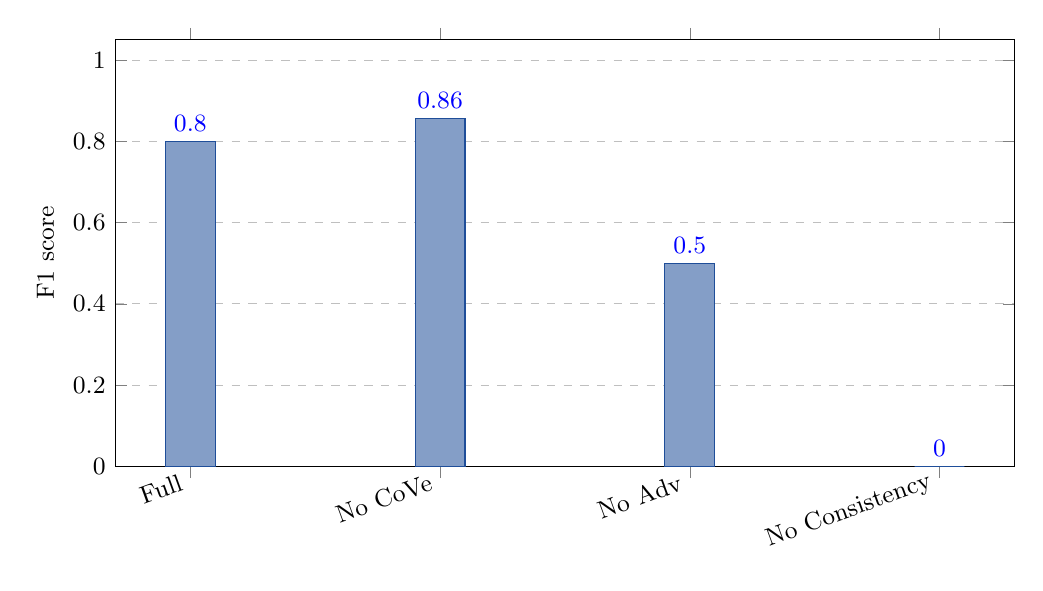
\begin{tikzpicture}[font=\small]
\begin{axis}[
  ybar,
  bar width=18pt,
  width=13cm,
  height=7cm,
  ymin=0,
  ymax=1.05,
  ylabel={F1 score},
  symbolic x coords={Full, No CoVe, No Adv, No Consistency},
  xtick=data,
  xticklabel style={rotate=20, anchor=east},
  nodes near coords,
  nodes near coords align={vertical},
  ymajorgrids=true,
  grid style=dashed,
]
\addplot+[fill=myblue!55, draw=myblue]
  coordinates {(Full,0.800) (No CoVe,0.857) (No Adv,0.500) (No Consistency,0.000)};
\end{axis}
\end{tikzpicture}
\caption{F1 score by ablation condition. No CoVe increases F1 on the small
sample, but Table~\ref{tab:confusion} shows that it does so by accepting one
false positive.}
\label{fig:f1-ablation}
\end{figure}

\begin{figure}[h!]
\centering
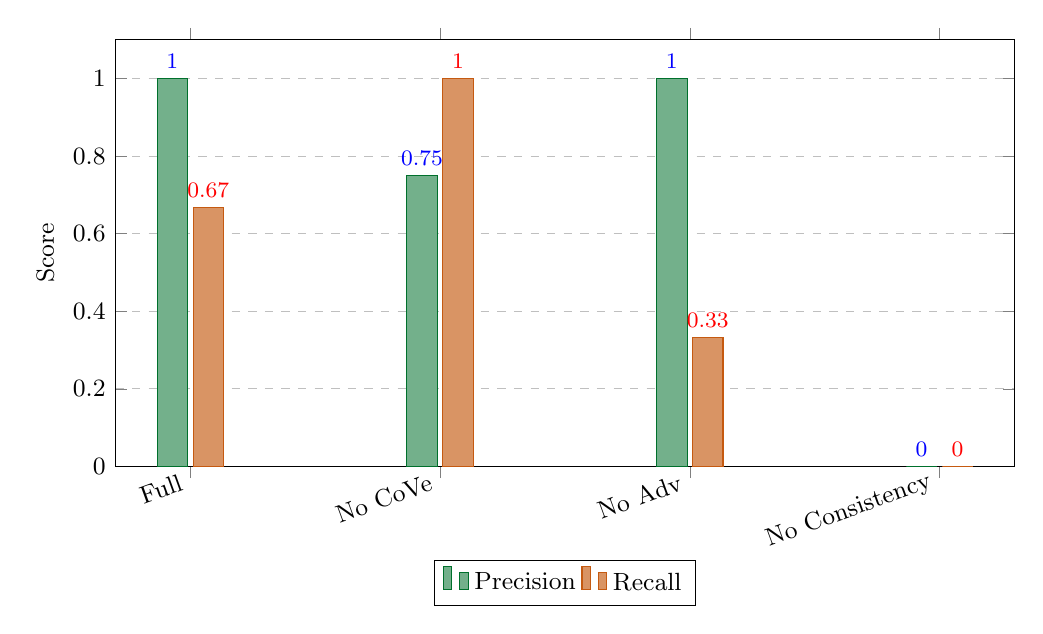
\begin{tikzpicture}[font=\small]
\begin{axis}[
  ybar,
  bar width=11pt,
  width=13cm,
  height=7cm,
  ymin=0,
  ymax=1.1,
  ylabel={Score},
  symbolic x coords={Full, No CoVe, No Adv, No Consistency},
  xtick=data,
  xticklabel style={rotate=20, anchor=east},
  legend style={at={(0.5,-0.22)}, anchor=north, legend columns=2},
  nodes near coords,
  nodes near coords align={vertical},
  every node near coord/.append style={font=\footnotesize},
  ymajorgrids=true,
  grid style=dashed,
]
\addplot+[fill=mygreen!55, draw=mygreen]
  coordinates {(Full,1.000) (No CoVe,0.750) (No Adv,1.000) (No Consistency,0.000)};
\addplot+[fill=myorange!65, draw=myorange]
  coordinates {(Full,0.667) (No CoVe,1.000) (No Adv,0.333) (No Consistency,0.000)};
\legend{Precision, Recall}
\end{axis}
\end{tikzpicture}
\caption{Precision and recall trade-off across ablations. CoVe improves
conservativeness by eliminating false positives, while adversarial retrieval is
important for recall.}
\label{fig:precision-recall}
\end{figure}

\section{Key Findings}

\textbf{Finding 1: CoVe enforces a precision-first correction policy.}
Full \sys{} obtains Precision = 1.000 and False Positive Rate = 0.000. This
means no clean paper in the sample was incorrectly flagged for correction. The
No-CoVe configuration reaches Recall = 1.000 but produces one false positive,
dropping precision to 0.750. The result supports CoVe as a conservative guard
rather than as a pure F1 maximizer.

\textbf{Finding 2: Adversarial retrieval validates the core thesis.}
Replacing adversarial queries with confirmatory queries reduces F1 from 0.800 to
0.500 and recall from 0.667 to 0.333. This is a 37.5\% relative F1 drop. The
result directly supports the claim that retrieval should search for possible
contradictions, not just related evidence.

\textbf{Finding 3: The consistency checker matters in the available run.}
The No-Consistency configuration reports zero true positives. Because this is a
five-paper sample, the result should be interpreted as diagnostic rather than
statistically conclusive. It nevertheless indicates that internal consistency is
part of the current system behavior and should be kept in future evaluations.

\section{Contextual Baseline Comparison}

Table~\ref{tab:baseline-context} places the five-paper \sys{} result beside
baseline numbers recorded in the project notes. These are contextual references
from published systems and are not direct head-to-head measurements on the same
SkepticBench sample.

\begin{table}[h!]
\centering
\caption{Contextual baseline comparison; datasets and protocols differ}
\label{tab:baseline-context}
\renewcommand{\arraystretch}{1.25}
\begin{tabularx}{\textwidth}{L{4.2cm} C{1.6cm} X}
\toprule
\textbf{System} & \textbf{F1} & \textbf{Source / Scope} \\
\midrule
\rowcolor{rowgray}
\sys{} (ours) & 0.800 & This work, SkepticBench sample ($N=5$ papers) \\
Standard RAG & 0.610 & Reference value from project notes based on Gao et al. \cite{gao2023} \\
\rowcolor{rowgray}
RARR & 0.710 & Reference value from project notes based on Gao et al. \cite{gao2023} \\
Zero-shot GPT-4 & 0.660 & Reference value from project notes based on Zheng et al. \cite{zheng2023} \\
\bottomrule
\end{tabularx}
\end{table}

\section{Interpretation}

The results should be read as an ablation proof-of-concept, not as a final
large-scale benchmark. The strongest evidence is internal: when one component is
removed, the system behavior changes in the direction predicted by the design.
Adversarial query removal hurts recall, while CoVe removal increases recall but
allows a false positive. This aligns with the intended architecture: adversarial
retrieval finds contradictions, and CoVe prevents weak contradiction claims from
becoming edits.


% ================================================================= %
%  CHAPTER 6: DISCUSSION AND LIMITATIONS
% ================================================================= %
\chapter{Discussion and Limitations}

\section{Discussion}
\label{Discussion}

The evaluation supports two design conclusions. First, adversarial retrieval is
not merely a prompt-style detail; it materially changes detection behavior. The
No-Adversarial configuration misses two of the three corrupted summaries, while
the full system detects two. This suggests that confirmatory search often
retrieves related context without surfacing the precise contradiction needed for
factual correction.

Second, CoVe should be evaluated according to the requirements of a correction
system. On the available sample, removing CoVe gives higher F1 because it
recovers the missed corrupted summary, but it also changes a clean case into a
false positive. If \sys{} were only a detector, that trade-off might be
acceptable. Because \sys{} edits text, the precision-first behavior of CoVe is
more appropriate: the system should avoid modifying correct summaries unless the
contradiction is well grounded.

The architecture is also useful from an engineering perspective. Each stage has
a clear failure boundary: retrieval can fail to find evidence, the judge can
return \texttt{INSUFFICIENT\_EVIDENCE}, CoVe can overturn weak contradictions,
and the editor can decline to change a sentence if it cannot identify a safe
replacement. This modularity makes the system auditable during demonstrations
and easier to improve component by component.

\section{Limitations}
\label{Limitations}

Despite promising ablation behavior, the current report has important
limitations:

\begin{itemize}
    \item \textbf{Small validated sample:} the reported ablation run contains five papers. The results are useful for design validation but not for statistical generalization.
    \item \textbf{Paper-level aggregation:} \texttt{results/ablation.json} stores paper-level counts, not the per-claim predictions needed for detailed error analysis.
    \item \textbf{Contextual baselines only:} Standard RAG, RARR, and zero-shot GPT-4 values are cited as external reference points, not as direct runs on the same SkepticBench sample.
    \item \textbf{Conflicting artifacts:} the root \texttt{results/ablation.json} and \texttt{Backend/results/ablation.json} contain different metrics. This report uses the root artifact because it matches the active \texttt{RESULTS\_SUMMARY.md}, but a final submission should archive one canonical run.
    \item \textbf{Retrieval dependency:} evidence quality depends on arXiv, Semantic Scholar, web search, cache state, and rate limits.
    \item \textbf{Domain specificity:} the system is tuned for AI/ML paper summaries and should not be presented as a general misinformation detector.
    \item \textbf{LLM dependence:} atomicization, judging, CoVe, and editing all depend on LLM behavior, so repeated runs may vary unless model versions and caches are fixed.
    \item \textbf{Venue and metadata errors:} some venue or publication-context claims are difficult to verify from abstracts alone and may require full-paper or proceedings-level evidence.
\end{itemize}


% ================================================================= %
%  CHAPTER 7: CONCLUSION AND FUTURE WORK
% ================================================================= %
\chapter{Conclusion and Future Work}

\section{Conclusion}
\label{Conclusion}

This project presents \sys{}, a skeptical hallucination detection and correction
pipeline for AI/ML paper summaries. The system combines atomic claim
decomposition, cross-claim consistency checking, adversarial retrieval, hybrid
evidence gathering, LLM judging, CoVe meta-verification, and surgical editing.
The central idea is that a verifier should actively search for evidence that
could falsify a claim, and a correction should be applied only when the judge's
contradiction decision is itself verified.

On the available SkepticBench sample of five papers, full \sys{} achieves
Precision = 1.000, Recall = 0.667, and F1 = 0.800 with zero false positives.
Removing CoVe increases recall to 1.000 and F1 to 0.857 but introduces a false
positive, showing the precision--recall trade-off. Removing adversarial queries
drops F1 to 0.500, validating the thesis that confirmatory retrieval is weaker
than adversarial falsification for hallucination detection.

The project is therefore report-ready as a focused prototype and ablation study,
provided the evaluation scale is stated honestly. Its main contribution is not a
claim of broad benchmark superiority, but a clear architecture and empirical
signal showing why adversarial retrieval and judge verification matter for
correction.

\section{Future Work}
\label{Future Work}

Future development should prioritize the following improvements:

\begin{itemize}
    \item \textbf{Canonical evaluation artifacts:} save per-paper and per-claim predictions for every run, including evidence quotes and correction spans.
    \item \textbf{Larger benchmark execution:} evaluate the full approximately 1.4k-entry CSV once API limits, caching, and retrieval stability are controlled.
    \item \textbf{Direct baseline runs:} run Standard RAG, RARR-style editing, and zero-shot judging on the same SkepticBench split for fair comparison.
    \item \textbf{Error-type analysis:} report performance separately for metric, date, author, venue, architecture, and training-objective hallucinations.
    \item \textbf{Human validation:} add manual annotation checks and inter-annotator agreement for ambiguous cases.
    \item \textbf{Retrieval hardening:} improve PDF-level extraction and proceedings/venue evidence retrieval for claims absent from abstracts.
    \item \textbf{Reproducibility controls:} pin model identifiers, cache snapshots, random seeds, and environment versions for final review submission.
    \item \textbf{Frontend demonstration:} connect the FastAPI backend and dashboard to show atomic facts, retrieved evidence, CoVe outcomes, and edits in a reviewer-friendly workflow.
\end{itemize}


% ================================================================= %
%  BIBLIOGRAPHY
% ================================================================= %
\begin{thebibliography}{99}

        \bibitem{dhuliawala2023} Dhuliawala, S., et al. (2023). Chain-of-Verification Reduces Hallucination in Large Language Models. \textit{arXiv:2309.11495}.

        \bibitem{gao2023} Gao, L., et al. (2023). RARR: Researching and Revising What Language Models Say, Using Language Models. \textit{arXiv:2210.08726}.

        \bibitem{min2023} Min, S., et al. (2023). FActScore: Fine-grained Atomic Evaluation of Factual Precision in Long Form Text Generation. \textit{arXiv:2305.14251}.

        \bibitem{chern2023} Chern, I. C., et al. (2023). FacTool: Factuality Detection in Generative AI. \textit{arXiv:2307.13528}.

        \bibitem{huang2023} Huang, J., et al. (2023). Deceptive Prompting: Exploiting the Sycophancy of Large Language Models. \textit{arXiv:2311.05684}.

        \bibitem{asai2023} Asai, A., et al. (2023). Self-RAG: Learning to Retrieve, Generate, and Critique through Self-Reflection. \textit{arXiv:2310.11511}.

        \bibitem{shinn2023} Shinn, N., et al. (2023). Reflexion: Language Agents with Verbal Reinforcement Learning. \textit{arXiv:2303.11366}.

        \bibitem{zhang2023} Zhang, M., et al. (2023). How Language Model Hallucinations Can Snowball. \textit{arXiv:2305.13534}.

        \bibitem{li2023} Li, J., et al. (2023). HaluEval: A Large-Scale Hallucination Evaluation Benchmark. \textit{arXiv:2305.11747}.

        \bibitem{wang2023} Wang, B., et al. (2023). Self-CheckGPT: Zero-Resource Hallucination Detection. \textit{arXiv:2308.11495}.

        \bibitem{peng2023} Peng, B., et al. (2023). Check Your Facts and Try Again: Improving Large Language Models with External Knowledge and Automated Feedback. \textit{arXiv:2302.12813}.

        \bibitem{mallen2023} Mallen, A., et al. (2023). When Not to Trust Language Models: Investigating Effectiveness of Parametric and Non-Parametric Memories. \textit{ACL}.

        \bibitem{liu2023} Liu, Y., et al. (2023). G-Eval: NLG Evaluation using GPT-4 with Better Human Alignment. \textit{arXiv:2303.16634}.

        \bibitem{wei2022} Wei, J., et al. (2022). Chain-of-Thought Prompting Elicits Reasoning in Large Language Models. \textit{NeurIPS}.

        \bibitem{yao2023} Yao, S., et al. (2023). ReAct: Synergizing Reasoning and Acting in Language Models. \textit{ICLR}.

        \bibitem{schick2023} Schick, T., et al. (2023). Toolformer: Language Models Can Teach Themselves to Use Tools. \textit{arXiv:2302.04761}.

        \bibitem{manakul2023} Manakul, P., et al. (2023). SelfCheckGPT: Zero-Resource Black-Box Hallucination Detection for Generative Large Language Models. \textit{EMNLP}.

        \bibitem{du2023} Du, Y., et al. (2023). Improving Factuality and Reasoning in Language Models through Multiagent Debate. \textit{arXiv:2305.14325}.

        \bibitem{zheng2023} Zheng, L., et al. (2023). Judging LLM-as-a-Judge on MT-Bench and Chatbot Arena. \textit{arXiv:2306.05685}.

        \bibitem{lightman2023} Lightman, H., et al. (2023). Let's Verify Step by Step. \textit{arXiv:2305.20050}.

        \bibitem{madaan2023} Madaan, A., et al. (2023). Self-Refine: Iterative Refinement with Self-Feedback. \textit{arXiv:2303.17651}.

        \bibitem{nakano2021} Nakano, R., et al. (2021). WebGPT: Browser-assisted question-answering with human feedback. \textit{arXiv:2112.09332}.

        \bibitem{lin2023} Lin, S., et al. (2023). TruthfulQA: Measuring How Models Mimic Human Falsehoods. \textit{ACL}.

        \bibitem{chen2023} Chen, Y., et al. (2023). FELM: Benchmarking Factuality Evaluation of Large Language Models. \textit{arXiv:2310.00741}.

        \bibitem{openai2023} OpenAI. (2023). GPT-4 Technical Report. \textit{arXiv:2303.08774}.

        \bibitem{touvron2023} Touvron, H., et al. (2023). Llama 2: Open Foundation and Fine-Tuned Chat Models. \textit{arXiv:2307.09288}.

    \end{thebibliography}
\end{document}
